% !TEX root = ejemplo.tex

\chapter{Compilación y arara}
Como este documento puede ser compilado con Lua\LaTeX{} o pdf\LaTeX{}, el
pdf de salida depende de qué tipo de compilación se usó,
entonces lo recomendable es que se si compila con un método y luego el otro
sea una compilación \enquote{nueva}, es decir, que antes de cambiar de
método se eliminen los archivos auxiliares para evitar posibles conflictos.

En este momento la compilación se ha vuelto algo complicada y por tanto puede
que tome algo de tiempo. Por ejemplo para generar la tabla de contenidos es
necesaria la siguiente cadena
\begin{flushleft}
  \verb|lualatex MiDocumento.tex|\\
  \verb|lualatex MiDocumento.tex|
\end{flushleft}

En la sección~\ref{sec:babel} ya se había mencionado cuál es la cadena de
compilación para obtener la bibliografía. Finalmente, para generar los
índices la compilación debe ser:
\begin{flushleft}
  \verb|lualatex MiDocumento.tex|\\
  \verb|makeindex MiDocumento.idx|\\
  \verb|lualatex MiDocumento.tex|
\end{flushleft}

Para ser más precisos se debería correr \texttt{makeindex} en cada índice que
se haya creado. En nuestro documento debería ser en el documento principal,
como arriba, para formar al índice alfabético y en \texttt{names.idx} para
formar el índice de nombres.

Si juntamos todos los pasos necesarios para obtener un pdf a partir de nuestros archivos, entonces obtenemos algo así:
\begin{flushleft}
  \verb|lualatex MiDocumento.tex|\\
  \verb|biber MiDocumento|\\
  \verb|makeindex MiDocumento.idx|\\
  \verb|lualatex MiDocumento.tex|\\
  \verb|lualatex MiDocumento.tex|
\end{flushleft}
donde, de nuevo, \texttt{makeindex} se debe correr en cada índice que se haya
creado. Como claramente tiene más pasos puede que haga el proceso algo lento.
Para hacer más rápida la compilación hay que evitar los pasos innecesarios.
Esto es, una vez que se ha compilado la primera vez se han creado los
archivos necesarios para componer bibliografía, índices, tabla de contenidos y
otros. Si no hay modificaciones a la bibliografía o índices, no es necesario
correr los pasos intermedios de arriba, ni tampoco correr tantas veces
\texttt{lualatex}. Para hacer esta compilación condicional escribimos
en las primeras líneas del archivo principal algo como lo siguiente
\begin{flushleft}
  \verb|% arara: ...|
\end{flushleft}
se usan para compilar con \texttt{arara} ya que se pueden agregar
condicionales de manera sencilla. Al menos mucho más simple que crear un
\texttt{latexmk} o un \texttt{makefile}. Aunque seguramente su instalación
local sí debe incluir \texttt{arara}, desgraciadamente overleaf no incluye
esta opción e ignorará los \textit{magic comments} del principio del archivo.

Con estos comandos sólo compilará la bibliografía cuando sea necesario, la
primera vez y cuando se modifiqué la bibliografía. De la misma forma sólo
compilara el índice alfabético cuando haga falta. En la primera compilación
de \texttt{lualatex} sólo creara los archivos auxiliares, ganando así un
poco de tiempo y las siguientes veces que corra \texttt{lualatex} activará
la opción \texttt{synctex} para que su editor y visor se comuniquen.

Ahora se compila con el comando
\begin{flushleft}
  \verb|arara MiDocumento|
\end{flushleft}
Para mostrar cómo mejoró el tiempo de compilación la segunda
vez ponemos capturas de pantalla de la compilación de este documento, ver figuras.
Además muchos editores de \LaTeX{} pueden configurarse para compilar con
\texttt{arara}.  Por ejemplo, en Atom (el editor que uso) con el paquete atom-
latex se configura como \textit{custom toolchain} y el toolchain es:
\begin{flushleft}
  \verb|arara %DOC -v|
\end{flushleft}

Para configurarlo en TeXMaker hay que seguir las instrucciones en
\url{https://tex.stackexchange.com/a/107995}.

En TeXWorks: \url{https://tex.stackexchange.com/a/98795}.

En TeXShop: \url{https://tex.stackexchange.com/a/175673}.

Un último comentario acerca del tiempo de compilación es que en el proceso
de revisión y correcciones de la tesis, por ejemplo al revisar un capítulo
específico donde no se requiera estar viendo los otros, se puede escribir en
el preámbulo \verb|\includeonly{CapituloEnRevision}|. Una vez que ya haya
sido compilado el documento completo el comando anterior hará que sólo se
compile el capítulo en revisión con la paginación y las referencias a otros
capítulos correctas. Esto podría mejorar mucho el tiempo de compilación.

\begin{figure}
\centering
  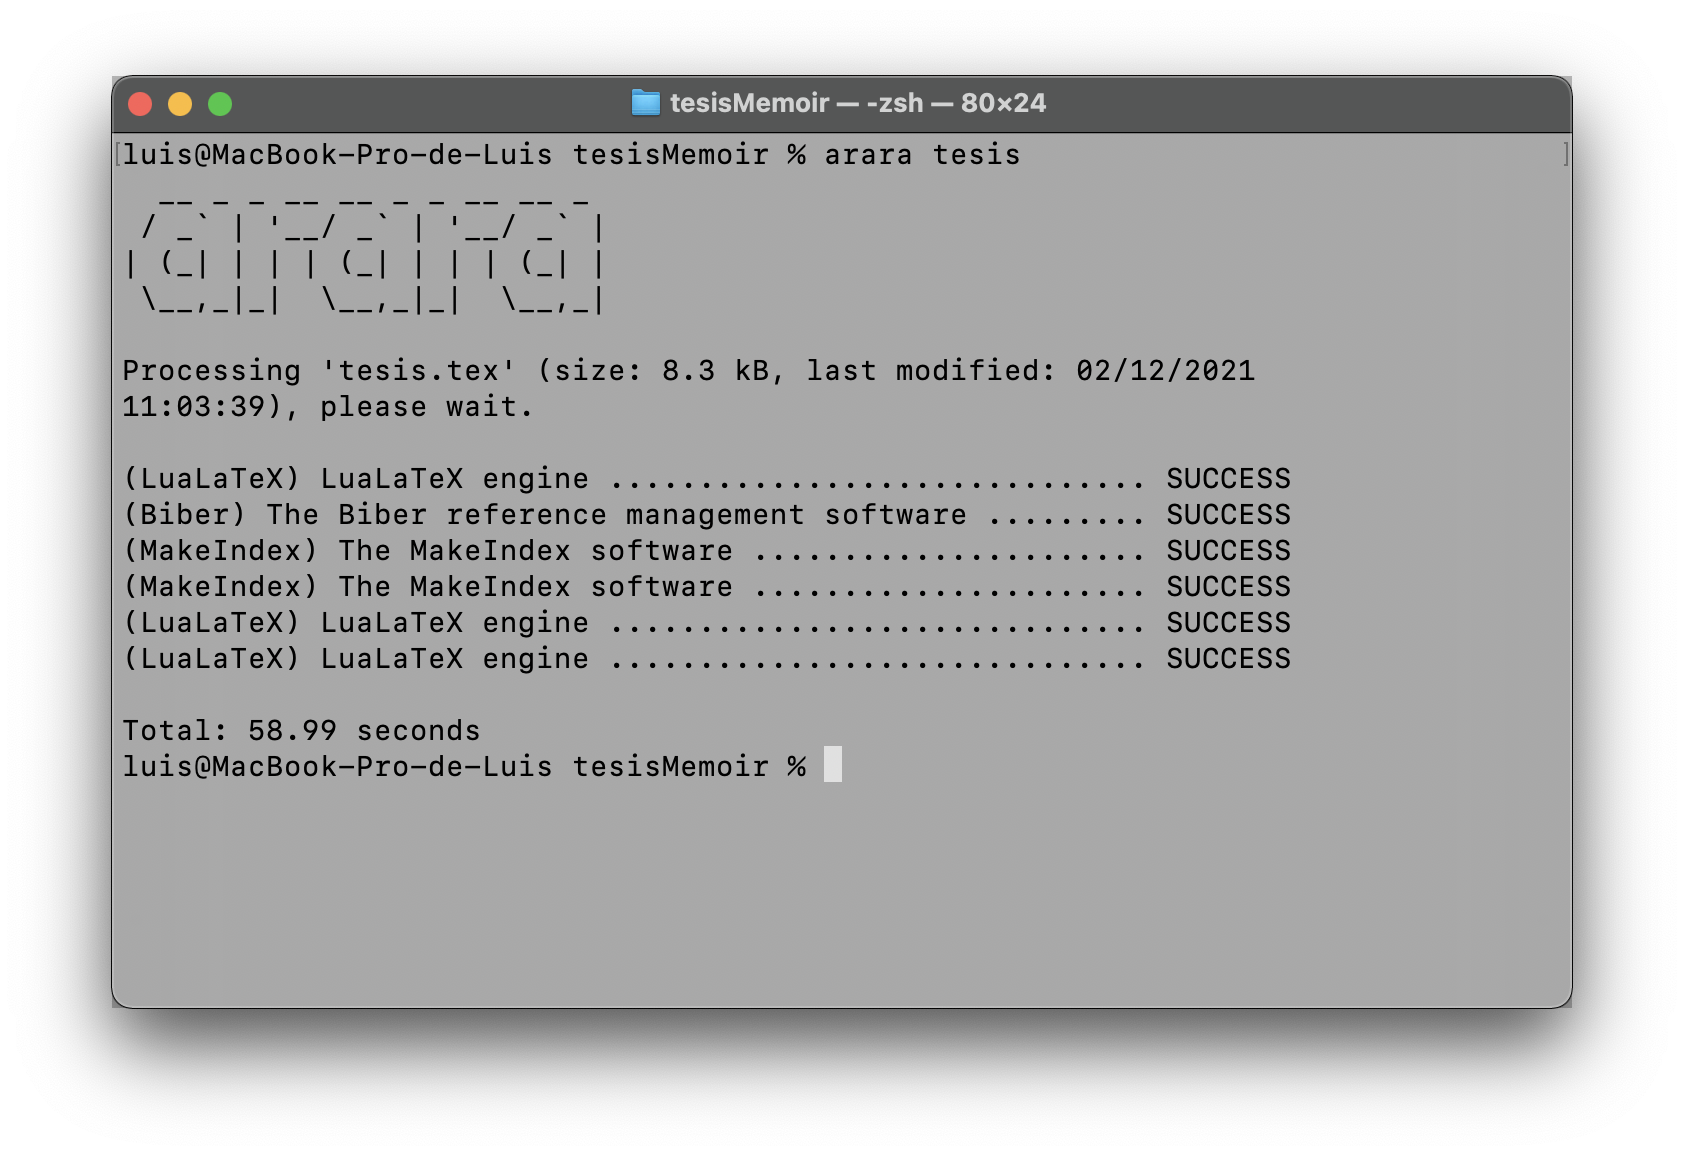
\includegraphics[scale=0.3]{primera}
  \caption{Primera compilación}
\end{figure}

\begin{figure}
\centering
  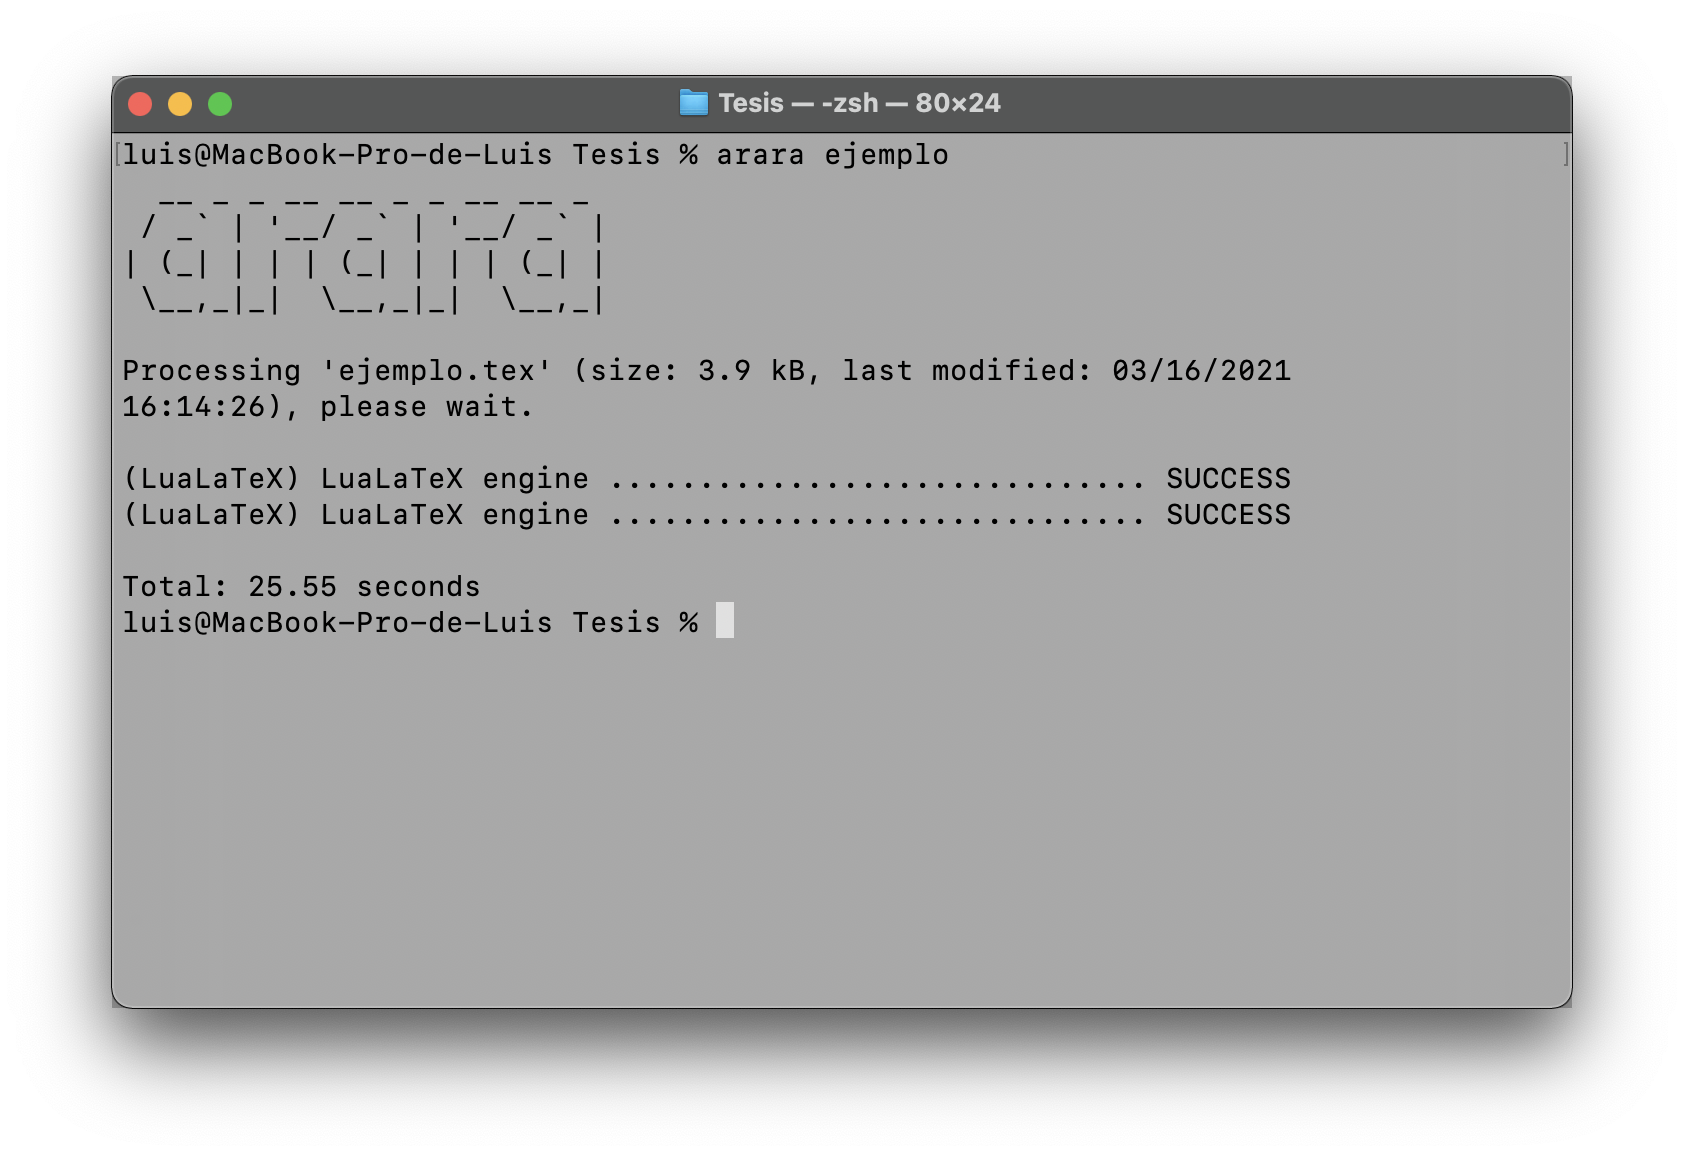
\includegraphics[scale=0.3]{segunda}
  \caption{Segunda compilación}
\end{figure}
